% !TeX root = ../../main.tex
\section{Ubi-Interact}\label{section:ubi-interact}
%\setcounter{footnote}{0} % for some reason, the footnote wants to start at 2

\gls{UBII} is a networking framework for distributed applications. Different devices connect to a centralized server, which manages the system in a local network. Every client can read and post data into channels (\enquote{Topics}) and execute code (\enquote{Interactions}) on the server. The protocol is extensible and platform-independent because \gls{Protobuf}\footnote{Protobuf is a mechanism to serialize data. The data is defined in a platform-neutral language, which compiles as a library to all commonly used programming languages~\cite{GoogleLLC.2019b}. Website: \href{https://developers.google.com/protocol-buffers/}{www.developers.google.com/protocol-buffers/}} is used to define it. The base components that build up the system are abstracted into Devices, Topics, and Interactions, which allows decoupling the implementation of software from device-specific environments.


\subsection{Architecture}\label{subsection:architecture}

The components of the \gls{UBII} framework, as visualized in Figure~\ref{fig:ubii-er}, are explained below.

\begin{figure}[H]
	\centering
	\begin{subfigure}[t]{.48\textwidth}
		\centering
		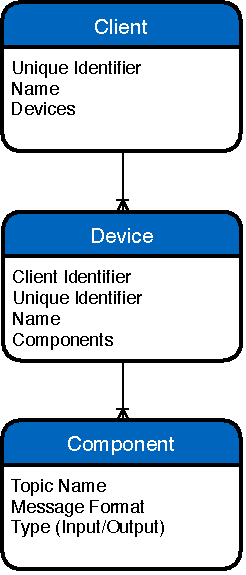
\includegraphics[height=6.5cm]{figures/implementation/ubii_er_client.pdf}
		\caption{The client components. A Client has multiple Devices, which has multiple Components.}\label{fig:ubii-er-client}
  \end{subfigure}%
  \hspace{0.04\textwidth}%
	\begin{subfigure}[t]{.48\textwidth}
		\centering
		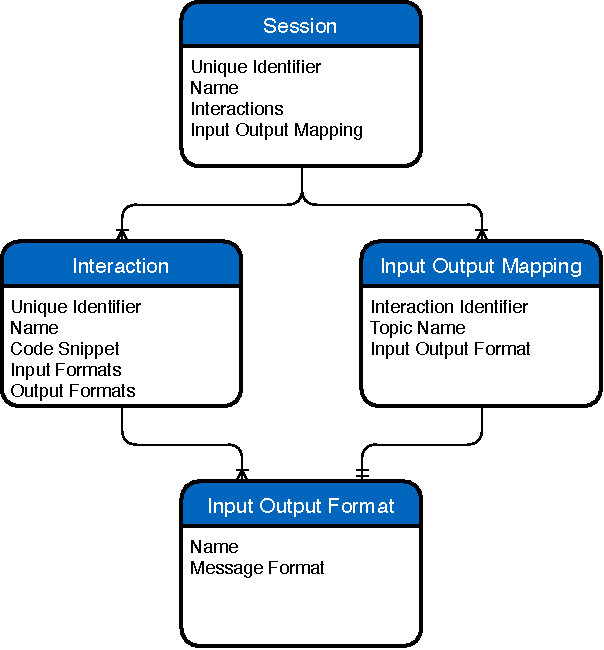
\includegraphics[height=6.5cm]{figures/implementation/ubii_er_server.pdf}
		\caption{The session components. A Session has multiple Interactions and Input Output Mappings. An Interaction has multiple Input Output Formats. The Input Output Mapping has one Input Output Format.}\label{fig:ubii-er-server}
	\end{subfigure}
	\caption[UBII components diagram]{The relationships of the core components in an entity relationship diagram.  Entities wich just contain a string are not shown for the sake of clarity.}\label{fig:ubii-er}
\end{figure}

\begin{description}
	\item[Server] or backend describes the centralized application which manages the connections. The Server is written in Node.js\footnote{Node.js is a JavaScript runtime. JavaScript is a programming language often used in web applications. Website: \href{https://nodejs.org/}{www.nodejs.org}}.
	\item[Clients] are basic network participants. They have to be registered on the Server before communication with other clients or the Server is possible. Clients are an abstraction of a physical network device and are defined by a \gls{UID}.
	\item[Devices] can be registered by Clients. A Device groups different input and output devices together. It is defined by a \gls{UID} and a list of Components. A data source for such an input device could be any sensor, for example, a button or a camera. Data output examples for input devices are lamps and displays.
	\item[Components] specify the Topic name, Message Formats for input/output devices and whether it publishes input or receives output data. 
	\item[Message Formats] defines the format of data published to a Topic. Even though it is possible to implement custom ones with \gls{Protobuf}, most common data types are already available. For example, \lstinline[mathescape=true]{Vector4$\times$4} (a four by four matrix), \lstinline{Vector2} (a two-dimensional vector) or \lstinline{boolean} (a binary value) are built-in. % chktex 46
	\item[Topics] are data channels which are addressed by a name. Clients can publish messages to Topics, which are registered by a Device. They can receive messages, after subscribing to a Topic. Such messages (also called \enquote{Topic Data}) are formatted as JSON\footnote{JSON is a standardized data exchange format, that uses human-readable text. It is often used for web-based data communication~\cite[iii]{ECMAInternational.2017}.}-string, whose structure is defined by the Message Formats.
	\item[Sessions] operate on the Server but are specified by the Client. They are defined by a \gls{UID} as well as a list of Interactions and mappings. The mappings (\enquote{Input/Output Mappings}) are defined by a Message Format and Topic name.
	\item[Interactions] are reactive components. They operate on Topics and are defined by a source code snippet\footnote{Currently, only JavaScript is supported as a programming language for Interactions, but Python is planned. Python is a programming language frequently used in scientific contexts. Website: \href{https://www.python.org/}{www.python.org}}. Interactions are executed in a fixed interval on the Server. They can subscribe to Topics and use the received Topic Data as input, given an Input/Output Mapping description. The output of the Interaction is published into another Topic. It is also possible to store data, which can be used in future executions (persistent state).
	\item[Services] are channels similar, used to send commands or requests to the Server. For example, they are used to subscribe to a Topic or list all available Topics.
\end{description}


\subsection{Interactions}\label{subsection:interactions}
A powerful feature of \gls{UBII} are Interactions. As explained in Chapter~\ref{subsection:architecture}, they are reactive components, which operate on Topics and regularly execute given code snippets on the Server. Interactions are isolated components, which depend on Topic Data. This abstraction introduces the possibility to reuse logic in other applications in a similar context. The data flow from a Device to the Interaction is visualized in the Figure~\ref{fig:ubii-cd}.

\begin{figure}[H]
	\centering
	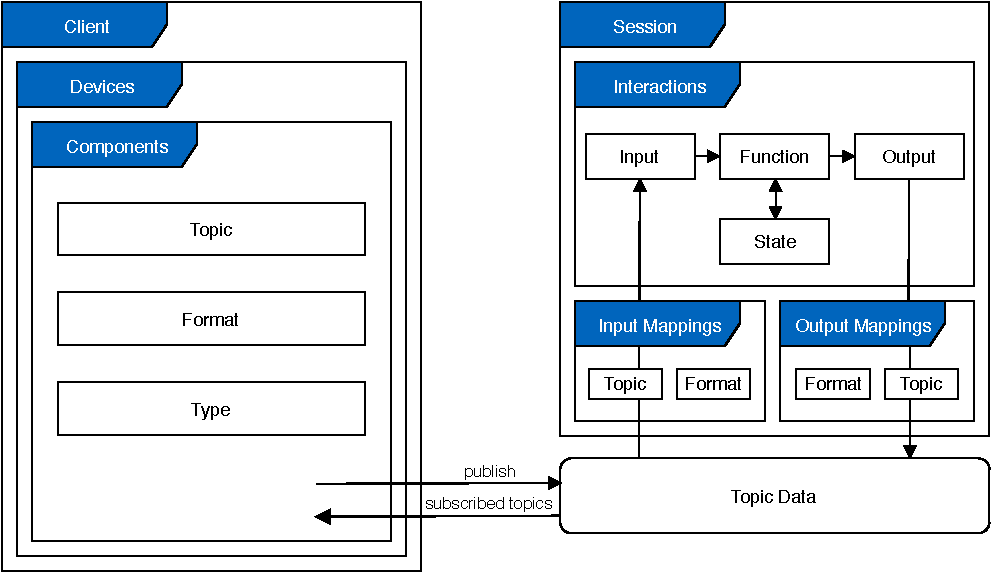
\includegraphics[width=12cm]{figures/implementation/ubii_cd.pdf}
	\caption[UBII communication diagram]{The interaction processing overview. This graphic gives a rough overview of the dataflow when using an Interaction. The diagram was created with the help of Sandro Weber. Rectangles represent entities, rounded rectangles represent data and arrows represent the data flow. The flow is described in detail in Chapter~\ref{subsection:architecture}.}\label{fig:ubii-cd}
\end{figure}

Interactions should be designed in an atomic and generic way so that they are easy to reuse. They can be used to discretize data, convert data to other formats, or to outsource logic from the application. Concrete examples include the detection of button presses, the transformation of coordinates, and the evaluation of data. An example of an Interaction which detects position changes can be seen in Figure~\ref{fig:ubii-interaction-example}.

\begin{figure}[H]
	\begin{lstlisting}[language=JavaScript]
    // detect intentional movement by comparing the current position with a previous one
    function(inputs, outputs, state) {
      const threshold = 0.05;

      if (state.lastPosition) {
        const vector = {
          x: inputs.position.x - state.lastPosition.x,
          y: inputs.position.y - state.lastPosition.y,
        };

        const squaredDistance = Math.pow(vector.x, 2) + Math.pow(vector.y, 2);

        outputs.moved = squaredDistance < threshold;
      } else {
        outputs.moved = true;
      }

      state.lastPosition = inputs.position;
    }
  \end{lstlisting}
	\caption[A UBII Interaction in JavaScript]{This is an example of an Interaction written in JavaScript. This Interaction calculates the squared distance of two points. One of the points is provided through the input, while the other one is stored in the state variable. The result of the comparison is then written into the output as a boolean data type. This is used to detect intended changes in the input position.}\label{fig:ubii-interaction-example}
\end{figure}

% this might be left out or merged into above
Another field of application would be to exchange data between two Topics, for example, to convert data from one format or unit to another one. An example of such a scenario could be an application, which consumes a rotation given in Euler angles. % replace however.. A problem might arise...
However, some input devices publish Euler angles in degrees. An Interaction, which takes Euler angles in degrees from one Topic and publishes Euler angles in radians to another one, could be implemented.

A code snippet, required to define an Interaction, has to define a function, which accepts three parameters:
\lstinline{inputs} is a collection of values, which were published into a Topic. The Topic is defined by the Input Mappings of the Session. \lstinline{outputs} is an empty collection, where values can be added. Those values are then published into a Topic, defined by the output mappings of the Session. \lstinline{state} stores a persistent collection of values, which can be used in later executions of the same Interaction.